\documentclass[a4paper]{proc}

\usepackage[utf8]{inputenc}
\usepackage[T1]{fontenc}
\usepackage[english]{babel}
\usepackage{graphicx}
\usepackage{url}

\author{Paul MABILEAU\\\texttt{paul.mabileau@telecom-sudparis.eu} \and Franck STAUFFER\\\texttt{franck.stauffer@telecom-sudparis.eu}}
\title{\textbf{Recursive Inter-Network Architecture's Security}}

\begin{document}
\maketitle
\tableofcontents
\newpage
\part*{Introduction}
The Recursive Inter-Network Architecture (RINA) is a network architecture based on Internet Process Communication (IPC) presented as an alternative to TCP/IP\@.
It was designed a while ago without security in mind. 
It has been patched to include security but it creates complexity.\cite{assessing-security}

\part{Comparing RINA against TCP/IP}
\section{Distibuted Application Facility}
The smallest part of RINA is the Distributed Application Process (DAP) which is a process running on a host, if at least two of them communicate it is called a Distributed Application Facility (DAF).
They communicate with objects structured in a Resource Information Base (RIB) that define naming and structure. (figure~\ref{daf})\\
They use a Common Distributed Application Protocol (CDAP) that permit to execute 6 operations on a distant DAP's objects:
\begin{itemize}
\item create
\item delete
\item read
\item start
\item stop
\item write
\end{itemize}
The DAF can be compared to the Application layer on the TCP/IP model. DAPs need underlying `layers' to communicate.\cite{wiki}

\begin{figure}
    \centering
    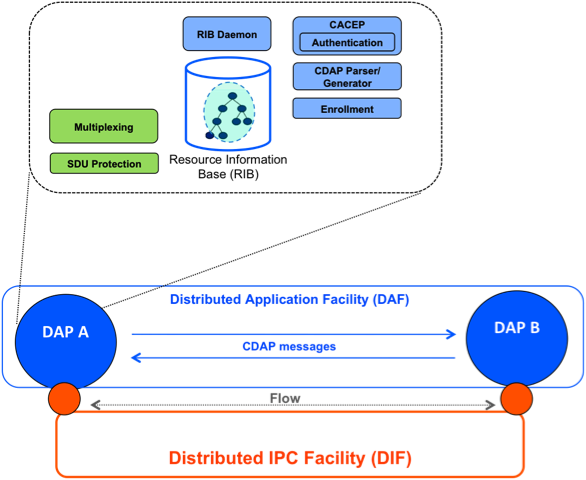
\includegraphics[width=0.9\columnwidth]{DAF.png}\label{daf}\caption{Base of RINA's architecture}
\end{figure}

\section{Distributed IPC Facility}
A Distributed IPC Facility (DIF) is a DAF but instead of containing DAPs, it contains IPC Processes (IPCPs).



\part{Security induced by RINA's conception}

\part{(optionnel) The threats to RINA}

\nocite{*}
\newpage
\bibliographystyle{unsrt}
\bibliography{report}
\end{document}
